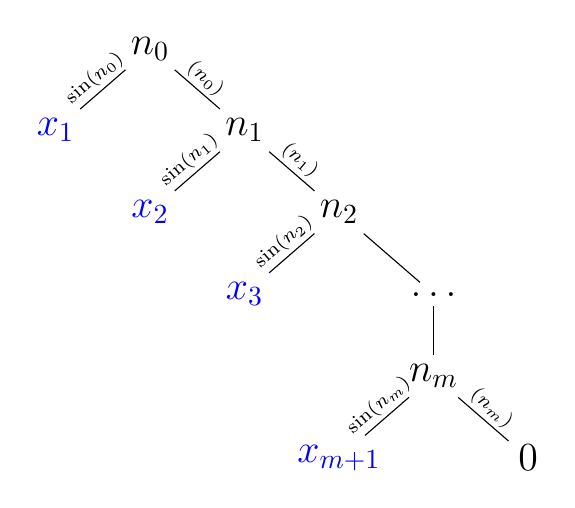
\begin{tikzpicture}[
		level distance=13mm,
		sibling distance=30mm,
		scale=0.8
		]
		\node {\Large$n_0$} 
		child {node[blue] {\Large$x_1$} 
			edge from parent node[xshift=-3,yshift=4,rotate=40.8] {\scriptsize$\sin(n_0)$}
		}
		child {node {\Large$n_1$}
			child {node[blue] {\Large$x_2$}
				edge from parent node[xshift=-3,yshift=4,rotate=40.8] {\scriptsize$\sin(n_1)$}  
			}
			child {node {\Large$n_2$}
				child {node[blue] {\Large$\phantom{n_1}x_{3}\phantom{n_1}$}
					edge from parent node[xshift=-3,yshift=4,rotate=40.8] {\scriptsize$\sin(n_2)$}  
				}
				child {node {\Large$\dots$}
				  	child {node {\Large$n_{m}$}
					child {node[blue] {\Large$x_{m+1}$}
						edge from parent node[xshift=-3,yshift=4,rotate=40.8] {\scriptsize$\sin(n_{m})$}
					}
					child {node {\Large$0$} edge from parent
						node[xshift=3,yshift=4,rotate=-40.8] {\scriptsize$\des(n_{m})$}}
				  }
				}
				edge from parent node[xshift=3,yshift=4,rotate=-40.8] {\scriptsize$\des(n_1)$}
			}
			edge from parent node[xshift=3,yshift=4,rotate=-40.8] {\scriptsize$\des(n_0)$}
		};
\end{tikzpicture}
